\documentclass{article}
\usepackage{tikz}
\usetikzlibrary{automata,positioning}

\begin{document}

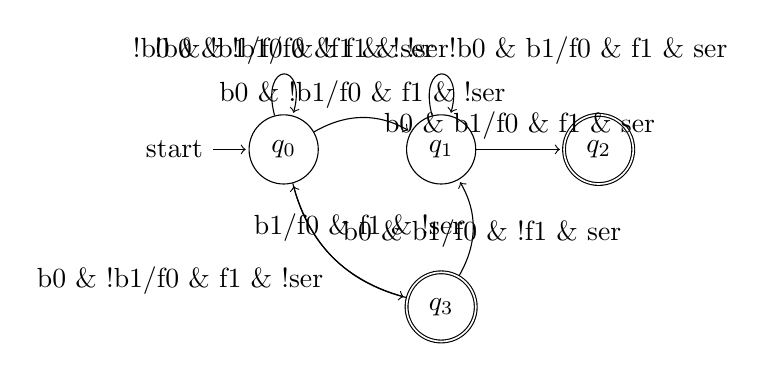
\begin{tikzpicture}[shorten >=1pt,node distance=2cm,on grid,auto]
    \node[state,initial] (q_0) {$q_0$};
    \node[state] (q_1) [right=of q_0] {$q_1$};
    \node[state,accepting] (q_2) [right=of q_1] {$q_2$};
    \node[state,accepting] (q_3) [below=of q_1] {$q_3$};

    \path[->]
        (q_0) edge [loop above] node {!b0 \& !b1/f0 \& !f1 \& !ser} ()
        (q_0) edge [bend left] node {b0 \& !b1/f0 \& f1 \& !ser} (q_1)
        (q_0) edge [bend right] node {b0 \& b1/f0 \& !f1 \& ser} (q_3)
        (q_1) edge [loop above] node {!b0 \& !b1/f0 \& f1 \& !ser\\!b0 \& b1/f0 \& f1 \& ser} ()
        (q_1) edge node {b0 \& b1/f0 \& f1 \& ser} (q_2)
        (q_3) edge [bend left] node {b0 \& !b1/f0 \& f1 \& !ser} (q_0)
        (q_3) edge [bend right] node {b1/f0 \& f1 \& !ser} (q_1);
\end{tikzpicture}

\end{document}